\documentclass[aps,pra,twocolumn,superscriptaddress,amsmath,amssymb,reprint]{revtex4-2}
\usepackage{graphicx}
\usepackage{bm}
\usepackage[colorlinks,allcolors=blue]{hyperref}
\newcommand{\Lc}{\mathcal L}
\newcommand{\Tr}{\operatorname{Tr}}
\begin{document}
\title{Finite-size decay-mode hybridization near a mean-field fold in an open Rydberg ensemble}
\author{[Author information to be completed]}
\noaffiliation
\date{\today}
\begin{abstract}
Mean-field multistability and the spectrum of a finite open quantum system describe different notions of degeneracy. We investigate their relation in a uniformly interacting Rydberg ensemble with independent local decay, retaining the full permutation-invariant operator space. On the monostable side of a mean-field fold, two real decay eigenvalues exhibit an avoided crossing with a rapidly decreasing finite-size gap. Physical product-state perturbations show that the high-branch relaxation response transfers between these modes across the crossing, while an oscillatory pair can decay more slowly than either real mode. A biorthogonal reduction identifies the normalization-invariant product of cross couplings that determines the gap; population tails alone do not determine its scaling. Eliminating nonzero coherence orders yields an exact spectral-parameter-dependent operator. The two decay eigenvalues are recovered as self-consistent roots of one effective eigenvalue branch, with full-generator residuals below $1.2\times10^{-13}\gamma$ for $N=24$--$48$. A local quadratic description reproduces the half-gap to relative errors decreasing from $1.2\%$ to $6.6\times10^{-6}$. We also verify exceptional points under complex-detuning continuation. These results establish a finite-size spectral description and its dynamical limits without identifying the observed gap exponent with a quasipotential or asserting an asymptotic fold correspondence.
\end{abstract}
\maketitle

\section{Introduction}
Nonlinear mean-field equations often provide the first description of bistability in driven open systems. Examples include optical and Rydberg ensembles, nonlinear resonators, and collective spin models~\cite{Carr2013,Casteels2017,Minganti2018,Xie2025}. A stable branch terminates at a saddle-node fold, whereas a finite quantum system evolves under a linear, trace-preserving Liouvillian. Relating these descriptions requires distinguishing roots of the stationary mean-field equations, eigenvalues of their Jacobian, and eigenvalues of the many-body generator.

This distinction is particularly relevant when exceptional points (EPs) are used to interpret nonlinear switching~\cite{SunYi2024,Xie2025}. A fold of stationary solutions need not be a defective eigenvalue of the mean-field Jacobian. Nor can a nontrivial Jordan block at zero describe the stationary sector of a finite-dimensional quantum dynamical semigroup: such a block would produce unbounded polynomial growth. Metastability instead involves small but nonzero decay eigenvalues and a separation of relaxation scales~\cite{Macieszczak2016,Minganti2018}.

Several parts of this connection are already understood. Switching between metastable attractors produces exponentially small rates, and quantum-instanton methods can predict these rates in collective spin systems, including models with local dissipation~\cite{PCE2026,CEP2026}. Few-mode descriptions of hysteresis have been developed~\cite{Krimer2019}. Cabot, Giorgi, and Zambrini identified a finite-size Liouvillian EP approaching a mean-field bifurcation and mediating between phase diffusion and quantum activation in a driven oscillator~\cite{Cabot2024}. These results motivate, but do not establish, an equivalent mechanism for a pair of modes whose common decay rate remains finite near a bistable fold.

Here we study such a pair in a uniformly interacting Rydberg model. Our focus is its finite-size spectral structure: which physical perturbations excite it, how its small splitting enters a non-Hermitian two-mode reduction, and what information is lost by eliminating quantum coherences without retaining spectral-parameter dependence. All new comparisons use the same double-precision generator. We restrict the quantitative claims to $\Omega=2\gamma$, $V=10\gamma$, and the sizes specified below.

We find an exchange of high-branch response between two real modes across an avoided crossing on the monostable side of the left fold. Their half-gap decreases approximately exponentially over $N=24$--$56$, but they are not always the two slowest decay modes. A biorthogonal reduction and an exact coherence-sector elimination provide complementary descriptions of the splitting. The latter exposes two self-consistent roots of a single effective eigenvalue branch and connects the slope of that branch to the biorthogonal norm of the full modes. These are applications of standard projection methods~\cite{Feshbach1958}; the model-specific result is the spectral and dynamical structure they resolve. We do not derive an asymptotic tunneling action or a universal fold-to-EP correspondence.

\section{Model, mean-field fold, and finite-size spectrum}
\label{sec:model}
We consider $N$ two-level atoms with excited-state number $\hat N_e=\sum_i\hat n_i$, collective spin $\hat J_\alpha=\frac12\sum_i\hat\sigma_i^\alpha$, and independent decay:
\begin{align}
 \dot\rho&=\Lc_N\rho=-i[\hat H,\rho]
 +\gamma\sum_i\mathcal D[\hat\sigma_i^-]\rho,\label{eq:L}\\
 \hat H&=-\Delta\hat N_e+\Omega\hat J_x
 +\frac{V}{2N}\hat N_e(\hat N_e-1),\label{eq:H}
\end{align}
where $\mathcal D[c]\rho=c\rho c^\dagger-\{c^\dagger c,\rho\}/2$. We set $\gamma=1$, so frequencies and eigenvalues below are measured in units of $\gamma$, and time in $\gamma^{-1}$.

Permutation invariance reduces the operator space to dimension $\binom{N+3}{3}$~\cite{Shammah2018}. We retain every Dicke $j$ block and the couplings between blocks caused by local decay; this is not a restriction to the maximum-spin sector. Throughout, ``full generator'' means the generator on this complete permutation-invariant operator space. This space contains the product states and observables considered here, but does not enumerate modes in other permutation-symmetry sectors.

In the large-$N$ factorized limit, writing the single-atom coherence as $\rho_{eg}=u+iv$ and the excited population as $n$, the mean-field equations are
\begin{align}
 \dot n&=-n-\Omega v,\nonumber\\
 \dot u&=-(\Delta-Vn)v-u/2,\label{eq:mf}\\
 \dot v&=(\Delta-Vn)u-\Omega(1-2n)/2-v/2.\nonumber
\end{align}
Their stationary populations satisfy
\begin{equation}
 F(n)=n[(\Delta-Vn)^2+1/4+\Omega^2/2]-\Omega^2/4=0.
 \label{eq:cubic}
\end{equation}
At $\Omega=2$, $V=10$, the left fold is at
\begin{equation}
 (\Delta_f,n_f)=(3.5996368905,\,0.1569270403).
\end{equation}
Using $F=\partial_nF=0$, the characteristic polynomial of the Bloch Jacobian at a fold reduces to
\begin{equation}
 \chi(\lambda)=\lambda[(\lambda+1)^2+\Omega^2/2].
 \label{eq:foldjac}
\end{equation}
Thus the zero eigenvalue is simple for the present nonzero drive. The identity also applies when the fold reaches the cusp: a triple root of the stationary cubic does not imply an EP3 of the Jacobian. The coalescing mean-field fixed points and the surviving high-population branch must also be distinguished; Eq.~\eqref{eq:foldjac} describes the former.

\begin{figure*}[t]
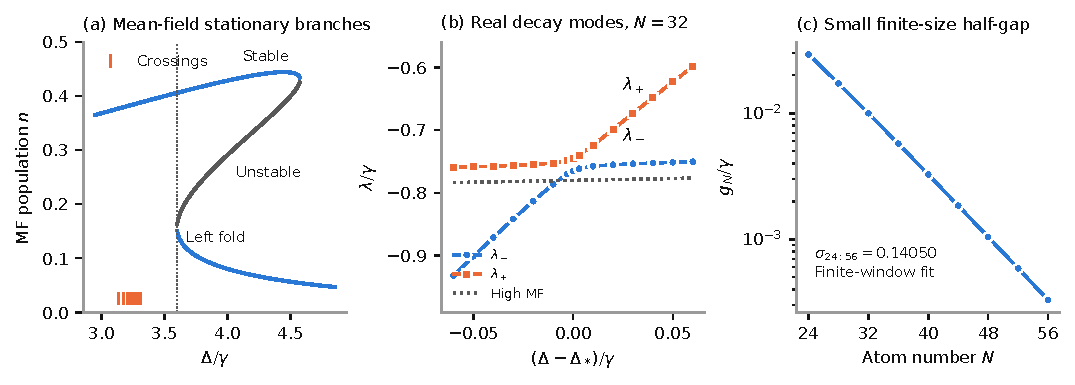
\includegraphics[width=\textwidth]{../figs/pra_spectrum.pdf}
\caption{Mean-field geometry and the finite-size real-mode crossing at $\Omega=2$, $V=10$. (a) Stationary populations: stable branches in blue, unstable branch in gray. Orange ticks mark the real-axis crossing positions for $N=24,28,\ldots,56$; all lie on the monostable side of the left fold. (b) The two target real eigenvalues for $N=32$, ordered as $\lambda_-<\lambda_+$, versus $\delta=\Delta-\Delta_*$. The dotted curve is the real relaxation eigenvalue of the surviving high mean-field branch. The modes exchange high-branch response, but the finite-size rates need not equal the mean-field rate. (c) Half-gap at its local minimum. The quoted exponent is a finite-window fit, not an established large-$N$ limit.}
\label{fig:spectrum}
\end{figure*}

We locate a local minimum of the separation between two real decay eigenvalues and denote it by $\Delta_*(N)$. Define
\begin{equation}
 g_N=\frac{\lambda_+(\Delta_*)-\lambda_-(\Delta_*)}{2}>0.
 \label{eq:gap}
\end{equation}
The positions move from $\Delta_*(24)=3.13740295$ to $\Delta_*(56)=3.30652148$, and the half-gap decreases from $0.0292933152$ to $0.000330979777$ [Fig.~\ref{fig:spectrum}]. A least-squares slope of $\ln g_N$ over $N=24,28,\ldots,56$ gives $\sigma_{24:56}=0.14050$. Restricting to $N=40$--$56$ gives $0.14305$, while successive four-atom slopes increase from $0.13218$ to $0.14383$. We therefore use ``approximately exponential'' only for the observed size window. The data do not determine a limiting exponent or prove $\Delta_*(N)\to\Delta_f$.

The small splitting must not be confused with a slow decay rate. At $N=32$ and $\Delta_*=3.205747775$, the real pair is
\begin{equation}
 \lambda_-=-0.765098904,\qquad \lambda_+=-0.745092273,
 \label{eq:realpair}
\end{equation}
whereas an oscillatory pair occurs at
\begin{equation}
 \lambda_{\rm osc}=-0.725036287\pm2.864794973i.
 \label{eq:oscpair}
\end{equation}
The oscillatory pair decays more slowly than both real modes. The target crossing is therefore not, in general, a crossing of the two slowest modes.

\section{Physical response and mode character}
\label{sec:modes}
A right eigenoperator is traceless and signed; its excitation-number profile is not a probability distribution. To test mode character without assigning identities solely from profile peaks, we evaluate signed spectral residues in a physical observable.

Let $R_i$ and $W_i$ be right and transpose-left eigenvectors of the stored generator, normalized by $W_i^TR_j=\delta_{ij}$. The transpose denotes the algebraic dual of the chosen vectorization. For the excitation-density observable $o^T\rho=\langle\hat N_e\rangle/N$, an initial difference $\delta\rho$ gives the exact contribution of a simple mode,
\begin{equation}
 \delta n_i(t)=a_i e^{\lambda_i t},\qquad
 a_i=(o^TR_i)(W_i^T\delta\rho).
 \label{eq:residue}
\end{equation}
Each residue is invariant under rescaling the corresponding left and right eigenvectors. The residues are signed and are not mode probabilities.

We use two preparations, specified in detail in the Supplemental Material (SM). The first is the difference of two positive product states displaced by $\pm\eta$ from the high mean-field fixed point along its real relaxation direction, with $\eta=0.005$. The second is a product state having the single-atom Bloch vector of the left fold, minus the exact finite-size stationary state at the chosen detuning. The latter is a controlled low-population preparation, not a finite-size metastable state assumed to exist outside the bistable interval.

For $N=32$, at $\delta=\Delta-\Delta_*=-0.06$, the high-branch perturbation has real-mode residues
\begin{equation}
 (a_-,a_+)=(8.94\times10^{-6},\,1.1694\times10^{-3}).
\end{equation}
At $\delta=+0.06$, they become
\begin{equation}
 (a_-,a_+)=(1.1082\times10^{-3},\,-2.91\times10^{-6}).
\end{equation}
The dominant high-branch response transfers from $\lambda_+$ to $\lambda_-$ [Fig.~\ref{fig:residues}(a)]. A separate $N=40$ calculation gives the same exchange, with the nondominant residue below $7.3\times10^{-7}$ at either endpoint. Halving $\eta$ changes the normalized residue vector by less than $7.3\times10^{-6}$ in relative Euclidean norm.

The fold-state preparation excites both modes and reveals large, opposite residues near the crossing [Fig.~\ref{fig:residues}(b)]. At $N=32$, $\delta=0$, they are approximately $(-1.666,1.423)$; at $N=40$ they are $(-5.475,5.217)$. Such values are allowed because individual spectral contributions can cancel. They do not imply that a physical density signal is unbounded.

The second diagnostic is the signed excitation-number profile $P_i(k)=\Tr(\Pi_kR_i)$. We measure its absolute-profile fraction in the region $k/N<0.22$, using the same fixed diagnostic cutoff on both sides. For $N=32$, the fractions change from $(0.209,0.0305)$ at $\delta=-0.06$ to $(0.0314,0.237)$ at $\delta=+0.06$ [Fig.~\ref{fig:residues}(c)]. Thus the branch with greater low-density support exchanges places with the high-branch response. Neither profile is purely localized in that region. We describe the second branch as having enhanced low-density character; a rigorous identification with a universal ghost-escape mode would require an independently controlled escape problem and is not assumed here.

\begin{figure*}[t]
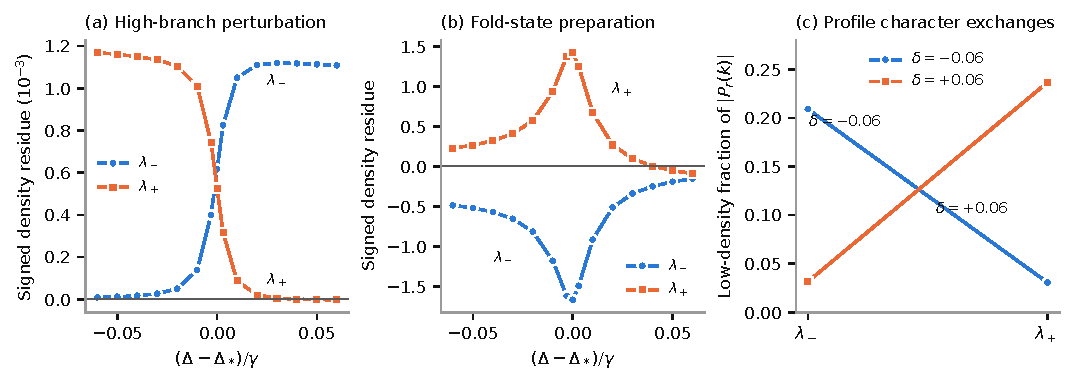
\includegraphics[width=\textwidth]{../figs/pra_residues.pdf}
\caption{Physical residues and exchange of mode character, $N=32$. (a) Residues of the two real modes in the excitation-density difference between product states displaced on opposite sides of the high mean-field fixed point. (b) Residues for a product state prepared at the left-fold Bloch vector, relative to the finite-size stationary state. Large opposite residues near the crossing cancel in the physical signal. (c) Fraction of the absolute excitation-number profile below $k/N=0.22$ at the two endpoints. This ratio is independent of mode normalization and characterizes the signed profile; it is not a population probability of a physical state.}
\label{fig:residues}
\end{figure*}

\section{Biorthogonal two-mode reduction and complex-detuning EPs}
\label{sec:two}
\subsection{Local reduction at the gap minimum}
Write $\Lc_N(\Delta)=L_0+\Delta L_1$, with $L_1\rho=i[\hat N_e,\rho]$. At $\Delta_*$, choose bases $R,W$ of the exact two-dimensional right and left invariant subspaces with $W^TR=I$. Diagonalizing $W^TL_1R$ defines a local diabatic basis with distinct real slopes $s_a,s_b$. Holding that basis fixed gives
\begin{equation}
 H_P(\delta)=
 \begin{pmatrix}e_a+s_a\delta&V_{ab}\\V_{ba}&e_b+s_b\delta\end{pmatrix},
 \qquad \delta=\Delta-\Delta_*.
 \label{eq:two}
\end{equation}
Here $a$ denotes the smaller-absolute-slope branch. At $\delta=0$ the projection is exact. Coupling to the complementary invariant subspace produces a spectral self-energy starting at order $\delta^2$ (SM); its small absolute size does not alone establish its smallness relative to an exponentially small coupling.

The squared separation at the projection point is
\begin{equation}
 d^2=(e_a-e_b)^2+4V_{ab}V_{ba},
 \qquad
 \partial_\Delta d^2=2(e_a-e_b)(s_a-s_b).
\end{equation}
At a nondegenerate minimum of a positive real gap, distinct slopes imply $e_a=e_b$ and hence
\begin{equation}
 \boxed{g_N^2=V_{ab}V_{ba}.}
 \label{eq:product}
\end{equation}
This identity uses the exact finite-size spectral subspace. It organizes the gap but is not an independent prediction of its exponent.

Under $R_i\mapsto c_iR_i$, $W_i\mapsto c_i^{-1}W_i$,
\begin{equation}
 V_{ab}\mapsto(c_b/c_a)V_{ab},\qquad
 V_{ba}\mapsto(c_a/c_b)V_{ba}.
\end{equation}
Individual coupling exponents can therefore depend on normalization if $c_i$ depend on $N$. We fix a population-peak convention, $\max_k|P_i(k)|=1$, with the largest-magnitude entry positive. Over $N=24$--$56$, the descriptive exponents are
\begin{align}
 \alpha_{ab}&=0.009638,\qquad \alpha_{ba}=0.271365,\nonumber\\
 (\alpha_{ab}+\alpha_{ba})/2&=0.140501.
\end{align}
Normalizing the right operators by their physical trace norm changes the first two values to $0.003563$ and $0.277440$, while preserving their sum. A balanced convention makes both equal to $\sigma$ by construction [Fig.~\ref{fig:couplings}]. Thus a directional exponent cannot be assigned an invariant activation interpretation from this decomposition alone.

\begin{figure*}[t]
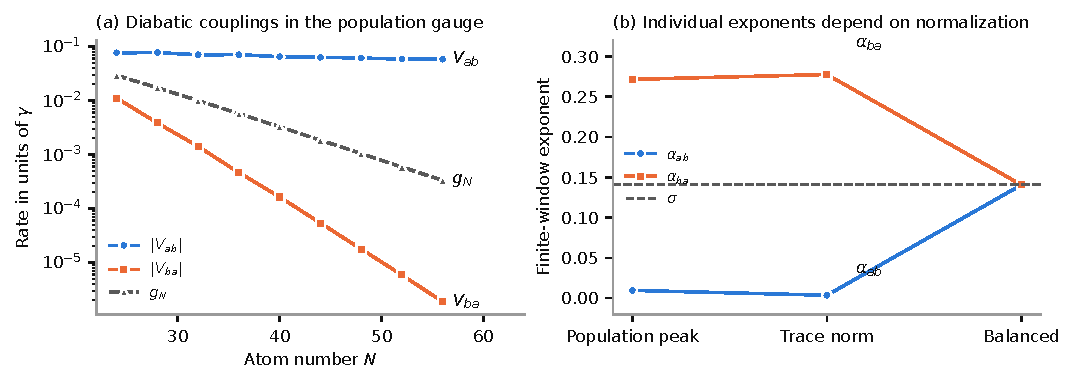
\includegraphics[width=\textwidth]{../figs/pra_couplings.pdf}
\caption{Biorthogonal gap decomposition. (a) Couplings in the population-peak convention, together with the invariant half-gap. (b) Finite-window exponents under three normalizations of the same two-dimensional subspace. The physical trace-norm convention changes the individual exponents; balancing the couplings makes each equal to $\sigma$ by construction. The invariant statement is their product and the sum of their logarithmic slopes.}
\label{fig:couplings}
\end{figure*}

The weak matrix element contains cancellations involving coherences. For $N=40$, summing its output-diagonal and output-off-diagonal contributions separately gives
\begin{equation}
 V_{ba}=0.9659542705-0.9657905699
       =1.63700625\times10^{-4}.
\end{equation}
This is not a representation-independent separation into two physical processes. Indeed, $W_b^T(L-cI)R_a=W_b^TLR_a$ for any scalar $c$, and choosing $c=e_a$ moves the cancellation into the small residual $(L-e_a)R_a$. The robust conclusion is that a right population tail by itself does not determine the full biorthogonal matrix element. A boundary-flux identity and its dependence on the chosen cut are given in the SM.

\subsection{Analytic continuation in detuning}
We separately continue the full generator as $L_0+\zeta L_1$ for complex detuning $\zeta$. This continuation uses $-i[H(\zeta),\rho]$; it is not $-i[H\rho-\rho H^\dagger]$. It remains trace preserving but is generally not Hermiticity preserving or CPTP.

A local two-subspace Newton calculation gives the upper-half-plane EP positions
\begin{align}
 \zeta_{\rm EP}(24)&=3.136806063+0.026370766i,\nonumber\\
 \zeta_{\rm EP}(32)&=3.205686613+0.007464558i,\label{eq:ep}\\
 \zeta_{\rm EP}(40)&=3.250218904+0.002129005i.\nonumber
\end{align}
At each point, the projected traceless matrix $M$ has nonzero norm, while $\|M^2\|_F/\|M\|_F^2<3.3\times10^{-15}$, consistent with a rank-one nilpotent. For $N=32$, analytic continuation around a circle of radius $0.00223937$ exchanges the two full-generator eigenvalues after one circuit and restores them after two. Changing the eigensolver seed and shift and doubling the sampling density preserves the result (SM).

The local linear model predicts $|\operatorname{Im}\zeta_{\rm EP}|\simeq2g_N/|s_a-s_b|$. The relative differences in the imaginary parts are $0.456\%$, $0.0792\%$, and $0.0115\%$ for $N=24,32,40$, respectively. This verifies nearby complex partners for the studied crossings; we do not claim that an arbitrary avoided crossing necessarily has a nearby EP. Nor does an EP in complex detuning constitute a physical degeneracy at real parameters.

\section{Exact elimination of coherence sectors}
\label{sec:coherence}
\subsection{Spectral-parameter-dependent effective operator}
To retain coherences without using full-generator eigenvectors as inputs, group the Dicke operator basis by signed coherence order $q=m-m'$. The diagonal Hamiltonian and local decay preserve $q$, whereas the drive connects only $q$ to $q\pm1$. The generator is therefore block tridiagonal in $q$.

Let $A_q=L_{q,q}$, $U_q=L_{q,q+1}$, and $D_q=L_{q+1,q}$. Starting at the highest positive order $Q=N$, define
\begin{align}
 \Sigma_Q(z)&=0,\nonumber\\
 \Sigma_{q-1}(z)&=U_{q-1}[zI-A_q-\Sigma_q(z)]^{-1}D_{q-1}.
 \label{eq:cf}
\end{align}
Here $z$ is an eigenvalue variable, distinct from the complex detuning $\zeta$ above. For real physical parameters and real $z$, Hermitian conjugation relates the positive and negative coherence chains. Their sum yields
\begin{equation}
 K_N(z)=A_0+2\operatorname{Re}\Sigma_0(z),\qquad
 K_N(z)r_0=zr_0.
 \label{eq:K}
\end{equation}
The $q=0$ sector still contains the populations of every Dicke block; it is not the excitation-number marginal alone, and $K_N(z)$ need not be a classical Markov generator.

With $P$ projecting onto $q=0$ and $Q=I-P$, the Schur identity reads
\begin{equation}
 \det(zI-L)=\det(zI-L_{QQ})\det[zI-K_N(z)].
 \label{eq:schur}
\end{equation}
It applies where $z-L_{QQ}$ is invertible; the recursion also requires invertible intermediate denominators. Purely coherent modes with zero $q=0$ projection and points at elimination poles require separate treatment. For complex $z$, the analytic continuation involves $\Sigma_+(z)+\overline{\Sigma_+(\bar z)}$, not $2\operatorname{Re}\Sigma_+(z)$. Our real-axis recursion is not used to compute Eq.~\eqref{eq:ep}.

The spectral dependence has a direct time-domain meaning. Eliminating $x_Q$ from the linear equations gives
\begin{align}
 \dot x_0(t)={}&L_{00}x_0(t)+L_{0Q}e^{tL_{QQ}}x_Q(0)\nonumber\\
 &+\int_0^t L_{0Q}e^{(t-s)L_{QQ}}L_{Q0}x_0(s)\,ds.
 \label{eq:memory}
\end{align}
Thus the self-energy represents memory carried by the eliminated coherence sectors. Replacing it by a constant is an additional approximation.

\subsection{Two roots of one effective branch}
In the local real spectral window, select a simple real eigenvalue branch $\mu_N(z)$ of $K_N(z)$ and define $f_N(z)=\mu_N(z)-z$. We find a negative local minimum,
\begin{align}
 f_N(z_c)&=-\epsilon_N<0,\qquad f_N'(z_c)=0,\nonumber\\
 c_N&=f_N''(z_c)>0.
\end{align}
Its two nearby roots give the two decay eigenvalues. Expanding around the minimum gives
\begin{equation}
 f_N(z)=-\epsilon_N+\frac{c_N}{2}(z-z_c)^2+\cdots,
 \qquad g_{N,\rm quad}=\sqrt{\frac{2\epsilon_N}{c_N}}.
 \label{eq:quadratic}
\end{equation}
The derivatives are calculated analytically through the matrix recursion and the non-Hermitian effective eigenproblem (SM).

\begin{table}[b]
\caption{Local real-axis coherence reduction. $g_N$ is the independently computed full-generator half-gap; the last column is $g_{N,\rm quad}/g_N-1$. All entries use $\gamma=1$.}
\label{tab:cf}
\begin{ruledtabular}
\begin{tabular}{rcccc}
$N$&$\epsilon_N$&$c_N$&$g_N$&Relative error\\
24&$9.33404\times10^{-3}$&22.28695&0.02929332&$-1.2002\times10^{-2}$\\
32&$1.09619\times10^{-3}$&21.96534&0.01000332&$-1.2773\times10^{-3}$\\
40&$1.28422\times10^{-4}$&24.11955&0.00326360&$-1.0842\times10^{-4}$\\
48&$1.51689\times10^{-5}$&27.82335&0.00104421&$-6.5891\times10^{-6}$
\end{tabular}
\end{ruledtabular}
\end{table}

For $N=24,32,40,48$, direct roots of $f_N=0$ reproduce the independent full-generator half-gaps to relative differences below $1.3\times10^{-9}$. Back-substituting all eight roots into the full generator gives $\|LR-zR\|_2/\|R\|_2<1.2\times10^{-13}$. Table~\ref{tab:cf} and Fig.~\ref{fig:coherence} show the separate, larger error of the quadratic approximation. The minimum location is not generally the midpoint of the two roots: at $N=24$, these are $z_c=-0.745502759$ and $(z_-+z_+)/2=-0.750910792$.

The two roots do not correspond to two nearby eigenvalues of a frozen $K_N(z_c)$. For $N=48$, its nearest eigenvalues include $-0.75910208$, $-0.21846755$, and zero, whereas the full generator has the two roots $-0.76013902$ and $-0.75805059$. The root pair is retained by self-consistency in $z$. This finding concerns this specific elimination; it does not rule out a different, correctly matched finite-dimensional effective model.

A four-point fit of $\ln\epsilon_N$ gives $\alpha_\epsilon=0.267635$, while the same convention applied to the curvature gives $\alpha_c=-0.009490$. Consequently the quadratic gap has fitted exponent $(\alpha_\epsilon-\alpha_c)/2=0.138562$, compared with $0.139030$ for the exact gap over the same four sizes. These are different fit windows from $\sigma_{24:56}$ above. No argument yet fixes the large-$N$ scaling of $\epsilon_N$ or proves that $c_N$ contributes only an algebraic prefactor. Equation~\eqref{eq:quadratic} is therefore a tested finite-size description, not an action-based exponent prediction.

\begin{figure*}[t]
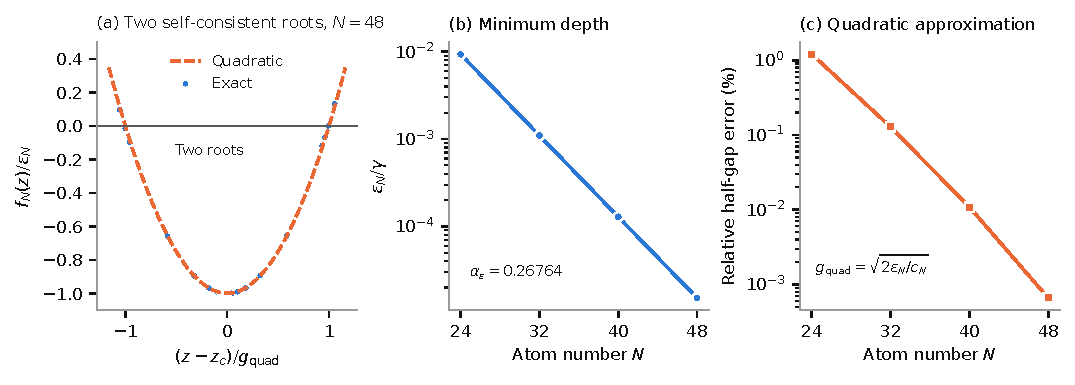
\includegraphics[width=\textwidth]{../figs/pra_coherence.pdf}
\caption{Exact coherence elimination at the supplied real-axis crossing detunings. (a) The normalized self-consistency function for $N=48$ (points) and its local quadratic expansion (dashed). (b) Negative-minimum depth and its descriptive four-size exponent. (c) Relative error of the quadratic half-gap. The exact eliminated roots have much smaller errors than this local expansion. Both the depth and curvature are outputs of a finite-$N$ spectral calculation; no independent large-$N$ action is inferred.}
\label{fig:coherence}
\end{figure*}

\subsection{Connection to biorthogonal self-orthogonality}
The effective spectral slope has a precise relation to the full-mode norm. Write $G=(zI-L_{QQ})^{-1}$, $B=L_{0Q}$, and $C=L_{Q0}$, so that $K=L_{00}+BGC$ and $K_z=-BG^2C$. For a simple effective eigenbranch with $Kr=\mu r$, $l^TK=\mu l^T$, and $l^Tr=1$, define the back-substituted vectors
\begin{equation}
 R=\binom{r}{GCr},\qquad W^T=(l^T,\,l^TBG).
\end{equation}
Then
\begin{equation}
 \boxed{W^TR=l^T(I-K_z)r=1-\mu_z=-f_z.}
 \label{eq:norm}
\end{equation}
These vectors are full eigenvectors only at a root. Away from it,
\begin{equation}
 (L-zI)R=\binom{f(z)r}{0},\qquad
 W^T(L-zI)=(f(z)l^T,0).
\end{equation}
Thus $f_z(z_c)=0$ at the observed negative minimum does not make $z_c$ an EP: $f(z_c)\ne0$, so it is not an eigenvalue.

For comparison, if the elimination is regular, the selected eigenvalue of $K(z_c)$ is algebraically simple, and $f=f_z=0$ with $f_{zz}\ne0$, Eq.~\eqref{eq:schur} implies an exactly double characteristic root. The kernel remains one-dimensional under back-substitution, giving an EP2. This conditional statement uses the analytic Schur operator and connects nonlinear spectral self-consistency to the usual defective-eigenvalue criterion. It does not supply the small depth $\epsilon_N$ in the present real-axis problem.

\section{Dynamical reach and limits of the real-mode pair}
\label{sec:dynamics}
Spectral hybridization does not ensure that two modes describe a measured transient. We compare Eq.~\eqref{eq:residue}, summed over the two real modes, with the action of $e^{tL}$ on the two physical initial differences used above. For $N=32$, we also include the oscillatory conjugate pair in Eq.~\eqref{eq:oscpair}. The time evolution is computed directly by sparse exponential multiplication, without fitting transient amplitudes or rates.

At the crossing, the relative $L^2$ error over $6\le t\le12$ for the high-branch preparation is $25.1\%$ with the two real modes and $0.506\%$ with all four modes. For the fold-state preparation the corresponding errors are $69.5\%$ and $5.00\%$. The latter initial condition has larger contributions from other modes and stronger cancellations; the same four-mode truncation need not be equally accurate for different preparations. On the two sides $\delta=\pm0.06$, the high-branch four-mode errors over the same window remain below $0.53\%$.

Figure~\ref{fig:dynamics} removes the common real-pair decay envelope only for visibility. Error definitions are in the SM, and the unscaled signals are supplied with the source data. The oscillatory pair is needed to account for the observed oscillations; omitting it leaves a substantial error even at late times. In particular, a small real-pair splitting does not by itself imply a long-lived physical response, since the pair's mean decay rate stays of order $\gamma$ over the studied sizes. These tests support a specific assignment of high-branch response and mode exchange, rather than a universal two-mode law for relaxation or chiral switching.

\begin{figure*}[t]
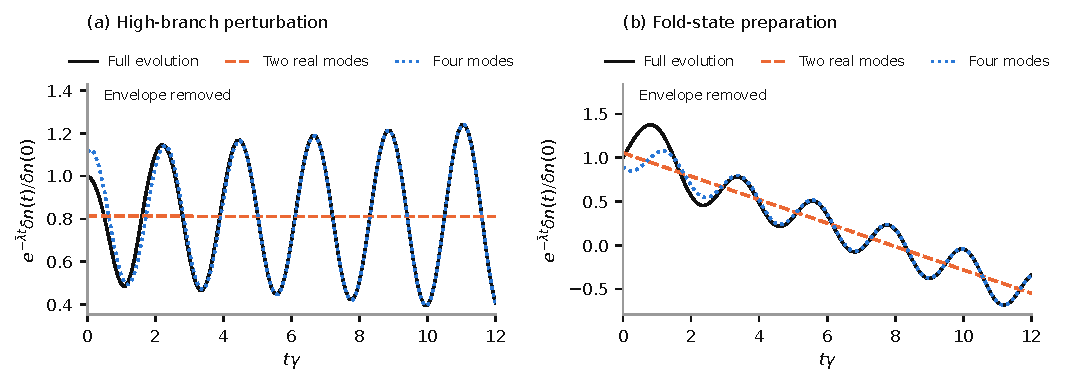
\includegraphics[width=\textwidth]{../figs/pra_dynamics.pdf}
\caption{Physical density transients at the $N=32$ crossing. Solid black: full permutation-invariant evolution. Orange dashed: the two target real modes with exact spectral residues. Blue dotted: those modes plus the oscillatory conjugate pair. (a) High-branch product-state perturbation; (b) fold-state preparation relative to the stationary state. The plotted signal is divided by its initial value and multiplied by $e^{-\bar\lambda t}$, with $\bar\lambda=(\lambda_-+\lambda_+)/2$, to expose spectral contributions after removing the common decay envelope. Errors quoted in the text are calculated from the unscaled signals.}
\label{fig:dynamics}
\end{figure*}

\section{Discussion and conclusions}
We have established a finite-size description of a real decay-mode avoided crossing on the monostable side of a mean-field Rydberg fold. The physical residue test shows exchange of high-branch relaxation response, supported by the simultaneous exchange of low-density profile character. This is stronger evidence than a visual assignment from population peaks, but does not identify a universal ghost-escape mode. The fold itself has a simple zero Jacobian eigenvalue, and the finite-size crossing involves modes with finite decay rates.

Two complementary reductions make the small gap precise. The exact two-dimensional spectral subspace gives the invariant product $V_{ab}V_{ba}=g_N^2$, while its directional factors depend on normalization and involve coherence-sensitive contractions. The coherence-sector Schur reduction recovers the two eigenvalues as self-consistent roots and provides an accurate local formula in terms of a minimum depth and curvature. Its spectral derivative also determines the full-mode biorthogonal norm. Complex-detuning EPs are separately verified by a regular invariant-subspace calculation and eigenvalue exchange, without treating the complex continuation as a physical generator.

The remaining asymptotic question is the origin of the small quantity $\epsilon_N/c_N$, or equivalently the invariant coupling product. A numerical proximity between a finite-window gap exponent and a stationary excitation-number rate function $\Phi(n_f)$ does not establish their equality. The stationary marginal discards information about left modes, coherence-sensitive residuals, and boundary matching. Quantum-instanton theory supplies a route to switching exponents~\cite{PCE2026,CEP2026}, but applying it to this finite-rate excited-mode splitting requires additional analysis. We make no quasipotential prediction here.

Our results also delimit the dynamical meaning of the spectral pair. An independently computed, more slowly decaying oscillatory pair substantially improves the density transient, demonstrating why the target real modes cannot simply be called the two slowest modes or assumed to govern every preparation. The present conclusions concern finite sizes and uniform interactions with local decay. They do not establish a thermodynamic-limit fold correspondence, extend to short-range nucleation, or provide a universal scaling law for direction-dependent switching.

\section*{Data and numerical methods}
The accompanying Supplemental Material specifies the generator convention, physical product-state construction, projection identities, root validation, and complex-continuation checks. The accompanying source bundle contains the plotted numerical records and reproduction scripts. The generator has been independently checked against the symmetrized full-spin Liouvillian for $N=1$--$4$. No fitted stochastic noise model is used in the finite-size spectral or transient calculations.

\begin{thebibliography}{99}
\bibitem{Carr2013} C. Carr, R. Ritter, C. G. Wade, C. S. Adams, and K. J. Weatherill, Nonequilibrium phase transition in a dilute Rydberg ensemble, Phys. Rev. Lett. \textbf{111}, 113901 (2013).
\bibitem{Casteels2017} W. Casteels, R. Fazio, and C. Ciuti, Critical dynamical properties of a first-order dissipative phase transition, Phys. Rev. A \textbf{95}, 012128 (2017).
\bibitem{Minganti2018} F. Minganti, A. Biella, N. Bartolo, and C. Ciuti, Spectral theory of Liouvillians for dissipative phase transitions, Phys. Rev. A \textbf{98}, 042118 (2018).
\bibitem{Xie2025} C. Xie, K. Sun, K.-D. Wu, C.-F. Li, G.-C. Guo, W. Yi, and G.-Y. Xiang, Chiral switching of many-body steady states in a dissipative Rydberg gas, Sci. Bull. \textbf{70}, 3345 (2025); arXiv:2402.02779.
\bibitem{SunYi2024} K. Sun and W. Yi, Encircling the Liouvillian exceptional points: a brief review, AAPPS Bull. \textbf{34}, 22 (2024).
\bibitem{Macieszczak2016} K. Macieszczak, M. Gu\c{t}\u{a}, I. Lesanovsky, and J. P. Garrahan, Towards a theory of metastability in open quantum dynamics, Phys. Rev. Lett. \textbf{116}, 240404 (2016).
\bibitem{PCE2026} K. Ptaszy\'nski, M. Chudak, and M. Esposito, Quantum instanton theory for metastable collective spin systems, arXiv:2604.15091 (2026).
\bibitem{CEP2026} M. Chudak, M. Esposito, and K. Ptaszy\'nski, Quantum instanton approach to metastable collective spin systems: Numerical implementation and applications, arXiv:2610.21684 (2026).
\bibitem{Krimer2019} D. O. Krimer and M. Pletyukhov, Few-mode geometric description of a driven-dissipative phase transition in an open quantum system, Phys. Rev. Lett. \textbf{123}, 110604 (2019).
\bibitem{Cabot2024} A. Cabot, G. L. Giorgi, and R. Zambrini, Nonequilibrium transition between dissipative time crystals, PRX Quantum \textbf{5}, 030325 (2024).
\bibitem{Feshbach1958} H. Feshbach, Unified theory of nuclear reactions, Ann. Phys. (N.Y.) \textbf{5}, 357 (1958).
\bibitem{Shammah2018} N. Shammah, S. Ahmed, N. Lambert, S. De Liberato, and F. Nori, Open quantum systems with local and collective incoherent processes: Efficient numerical simulations using permutational invariance, Phys. Rev. A \textbf{98}, 063815 (2018).
\end{thebibliography}
\end{document}
